
%TOdo: Vertalen
\chapter{OWASP top 10}\label{ch:owasp-top-10}
%TODO: Uitwijden over wat de owasp is.
\section{Wat is de OWASP}
Het Open Web Application Security Project® (OWASP) is een stichting zonder winstoogmerk die zich inzet voor het verbeteren van de beveiliging van software. Door middel van door de gemeenschap geleide open-source softwareprojecten, honderden lokale afdelingen over de hele wereld, tienduizenden leden en toonaangevende onderwijs- en trainingsconferenties, is de OWASP Foundation de bron voor ontwikkelaars en technologen om het web te beveiligen.

Hulpmiddelen en bronnen
Gemeenschap en netwerken
Onderwijs en opleiding

Al bijna twintig jaar ondersteunen bedrijven, stichtingen, ontwikkelaars en vrijwilligers de OWASP Foundation en haar werk. Doneer, word lid of word vandaag nog zakelijk lid.

\section{OWASP top 10}\label{sec:owasp-top-10}
De OWASP top 10 wordt iedere 5 jaar uitgebracht om aan te geven wat de belangrijkste punten van aandacht zijn op het gebied van het veilig ontwikkelen van software. Met als doel om awareness te generen en zo software nog veiliger te maken. Hieronder staat een vrij vertaalde versie die op de website te vinden is. Zoals te zien is in figuur~\ref{fig:OWASPTop10Shifts} veranderd de focus iedere keer wat inhoud dat er werk gedaan wordt maar er nog steeds werk moet worden verricht.
\begin{figure}[bth]
    \myfloatalign
    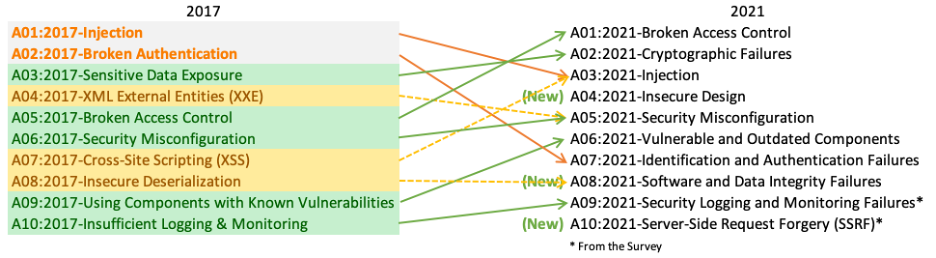
\includegraphics[width=10cm]{gfx/OWASPTop10 2017 to 2021}
    \caption{Verschuivingen OWASP Top 10 van 2017 naar 2021}
    \label{fig:OWASPTop10Shifts}
\end{figure}
\subsection{methode}
Om de top-10 samen te stellen wordt er gekeken naar de kwetsbaarheden gemeld in een CVE database. Waarbij er een gemiddelde wordt genomen van de exploit en impact score

In 2017, we selected categories by incidence rate to determine likelihood, then ranked them by team discussion based on decades of experience for Exploitability, Detectability (also likelihood), and Technical Impact. For 2021, we want to use data for Exploitability and (Technical) Impact if possible.

We downloaded OWASP Dependency Check and extracted the CVSS Exploit, and Impact scores grouped by related CWEs. It took a fair bit of research and effort as all the CVEs have CVSSv2 scores, but there are flaws in CVSSv2 that CVSSv3 should address. After a certain point in time, all CVEs are assigned a CVSSv3 score as well. Additionally, the scoring ranges and formulas were updated between CVSSv2 and CVSSv3.

In CVSSv2, both Exploit and (Technical) Impact could be up to 10.0, but the formula would knock them down to 60% for Exploit and 40% for Impact. In CVSSv3, the theoretical max was limited to 6.0 for Exploit and 4.0 for Impact. With the weighting considered, the Impact scoring shifted higher, almost a point and a half on average in CVSSv3, and exploitability moved nearly half a point lower on average.

There are 125k records of a CVE mapped to a CWE in the National Vulnerability Database (NVD) data extracted from OWASP Dependency Check, and there are 241 unique CWEs mapped to a CVE. 62k CWE maps have a CVSSv3 score, which is approximately half of the population in the data set.

For the Top Ten 2021, we calculated average exploit and impact scores in the following manner. We grouped all the CVEs with CVSS scores by CWE and weighted both exploit and impact scored by the percentage of the population that had CVSSv3 + the remaining population of CVSSv2 scores to get an overall average. We mapped these averages to the CWEs in the dataset to use as Exploit and (Technical) Impact scoring for the other half of the risk equation.
\subsection{Top 10}\label{subsec:top-10}
% TODO: door Google Translate halen
\begin{itemize}
    \item \textbf{A01:2021-Broken Access Control} moves up from the fifth position to the category with the most serious web application security risk; the contributed data indicates that on average, 3.81\% of applications tested had one or more Common Weakness Enumerations (CWEs) with more than 318k occurrences of CWEs in this risk category. The 34 CWEs mapped to Broken Access Control had more occurrences in applications than any other category.
    \item \textbf{A02:2021-Cryptographic Failures} shifts up one position to #2, previously known as A3:2017-Sensitive Data Exposure, which was broad symptom rather than a root cause. The renewed name focuses on failures related to cryptography as it has been implicitly before. This category often leads to sensitive data exposure or system compromise.

    \item \textbf{A03:2021-Injection} slides down to the third position. 94\% of the applications were tested for some form of injection with a max incidence rate of 19\%, an average incidence rate of 3.37\%, and the 33 CWEs mapped into this category have the second most occurrences in applications with 274k occurrences. Cross-site Scripting is now part of this category in this edition.

    \item \textbf{A04:2021-Insecure Design} is a new category for 2021, with a focus on risks related to design flaws. If we genuinely want to "move left" as an industry, we need more threat modeling, secure design patterns and principles, and reference architectures. An insecure design cannot be fixed by a perfect implementation as by definition, needed security controls were never created to defend against specific attacks.

    \item \textbf{A05:2021-Security Misconfiguration} moves up from #6 in the previous edition; 90\% of applications were tested for some form of misconfiguration, with an average incidence rate of 4.5\%, and over 208k occurrences of CWEs mapped to this risk category. With more shifts into highly configurable software, it's not surprising to see this category move up. The former category for A4:2017-XML External Entities (XXE) is now part of this risk category.

    \item \textbf{A06:2021-Vulnerable and Outdated Components} was previously titled Using Components with Known Vulnerabilities and is #2 in the Top 10 community survey, but also had enough data to make the Top 10 via data analysis. This category moves up from #9 in 2017 and is a known issue that we struggle to test and assess risk. It is the only category not to have any Common Vulnerability and Exposures (CVEs) mapped to the included CWEs, so a default exploit and impact weights of 5.0 are factored into their scores.

    \item \textbf{A07:2021-Identification and Authentication Failures} was previously Broken Authentication and is sliding down from the second position, and now includes CWEs that are more related to identification failures. This category is still an integral part of the Top 10, but the increased availability of standardized frameworks seems to be helping.

    \item \textbf{A08:2021-Software and Data Integrity Failures} is a new category for 2021, focusing on making assumptions related to software updates, critical data, and CI/CD pipelines without verifying integrity. One of the highest weighted impacts from Common Vulnerability and Exposures/Common Vulnerability Scoring System (CVE/CVSS) data mapped to the 10 CWEs in this category. A8:2017-Insecure Deserialization is now a part of this larger category.

    \item \textbf{A09:2021-Security Logging and Monitoring Failures} was previously A10:2017-Insufficient Logging & Monitoring and is added from the Top 10 community survey (#3), moving up from #10 previously. This category is expanded to include more types of failures, is challenging to test for, and isn't well represented in the CVE/CVSS data. However, failures in this category can directly impact visibility, incident alerting, and forensics.

    \item \textbf{A10:2021-Server-Side Request Forgery} is added from the Top 10 community survey (#1). The data shows a relatively low incidence rate with above average testing coverage, along with above-average ratings for Exploit and Impact potential. This category represents the scenario where the security community members are telling us this is important, even though it's not illustrated in the data at this time

\end{itemize}
